\documentclass[a4paper,landscape,12pt]{article}
\usepackage[svgnames]{xcolor}
\usepackage{wallpaper}
\usepackage{ragged2e}
\usepackage{ulem}
\usepackage{etoolbox}
\usepackage[object=pgfhan]{pgfornament}
\usetikzlibrary{chains}
\usetikzlibrary{calc}
\usetikzlibrary{decorations}
\usetikzlibrary{decorations.text,decorations.markings}
\usetikzlibrary {decorations.pathmorphing,shadows}

\usepackage{geometry}
\geometry{hmargin=1in,vmargin=0.8in,headheight=10pt}

\usepackage{fancyhdr}
\fancyhf{}
\renewcommand{\headrule}{}

\fancyhead[L]{%
\newpgfornamentfamily{pgfhan}
\begin{tikzpicture}[overlay,remember picture]
    \tikzset{every node/.append style={inner sep=0pt,color=MidnightBlue!50}}
    \tikzset{pgfornamentstyle/.style={draw=green!20!black,
    fill=orange,fill opacity=.5,thick}}%
    \newbox{\fortyseven}
\savebox{\fortyseven}{\pgfornament[scale=0.50]{32}}
    \node[anchor=north west,shift={(14.5pt,-14.5pt)}] at (current page.north west)
  (nw) {\pgfornament[scale=0.5]{12}};
    \node[anchor=north east,shift={(-14.5pt,-14.5pt)}] at (current page.north east)
    (ne) {\pgfornament[scale=0.5,symmetry=v]{12}};
  \node[anchor=south west,shift={(14.5pt,14.5pt)}] at (current page.south west)
    (sw) {\pgfornament[scale=0.5,symmetry=h]{12}};
  \node[anchor=south east,shift={(-14.5pt,14.5pt)}] at (current page.south east)
    (se) {\pgfornament[scale=0.5,symmetry=c]{12}};
%    \pgfornamentline[scale=0.25,shift={(0pt,-14.5pt)}]{nw.north west}{ne}{20}{32};
% \begin{scope}[start chain,node distance=-1pt]
%     \node[anchor=north west,on chain] at (nw.north east)
%     {\usebox{\fortyseven}};
%     \foreach \i in {1,...,9} {\node[on chain]{\usebox{\fortyseven}};}
%     \end{scope}
\foreach \i in {0,...,6}
   \node[anchor=north west,shift={($\i*(100bp,0)-(50bp,0)$)}] at (nw.north east)
    {\usebox{\fortyseven}};
\foreach \i in {0,...,3}
    \node[anchor=south east,shift={($\i*(0,-100bp)$)},rotate=90] at (ne.south east)
     {\usebox{\fortyseven}};
\foreach \i in {0,...,6}
     \node[anchor=south west,shift={($\i*(100bp,0)-(50bp,0)$)}] at (sw.south east)
      {\usebox{\fortyseven}};
\foreach \i in {0,...,3}
      \node[anchor=south west,shift={($\i*(0,-100bp)$)},rotate=-90] at (nw.south west)
       {\usebox{\fortyseven}};
   %         \foreach \i in {0,...,22}
% \node[anchor=south west,rotate=-90,
% shift={($\i*(31bp,0)$)}] at (nw.south west)
% {\usebox{\fortyseven}};
    %   \node[anchor=north west] at (nw.north east) {\pgfornament[scale=0.25]{32}};
%    \draw [scale=0.25] (nw) to [ornament=12] (ne);
%   \node[anchor=north west] at (nw.north east)%
%     {\pgfornament[scale=0.25]{32}};
%     \node[anchor=south west] at (sw.south east)%
%     {\pgfornament[scale=0.25]{32}};
%     \node[anchor=south west,rotate=-90] at (nw.south west)
%     {\pgfornament[scale=0.25]{32}};
%     \node[anchor=south east,rotate=90] at (ne.south east)
%     {\pgfornament[scale=0.25]{32}};
%     \node[anchor=center,shift={(25bp,-25bp)}] at (nw.south east)
%     {\pgfornament[scale=0.5]{57}};
\end{tikzpicture}
}

% \node[anchor=north west,shift={(14.5pt,-14.5pt)}] at (current page.north west)
%   (nw) {\pgfornamenthan[scale=0.2]{25}};

\pagestyle{fancy}
\fancypagestyle{plain}{\pagestyle{fancy}}

\usepackage{environ}

\NewEnviron{myframe}{%
\newpgfornamentfamily{vectorian}
    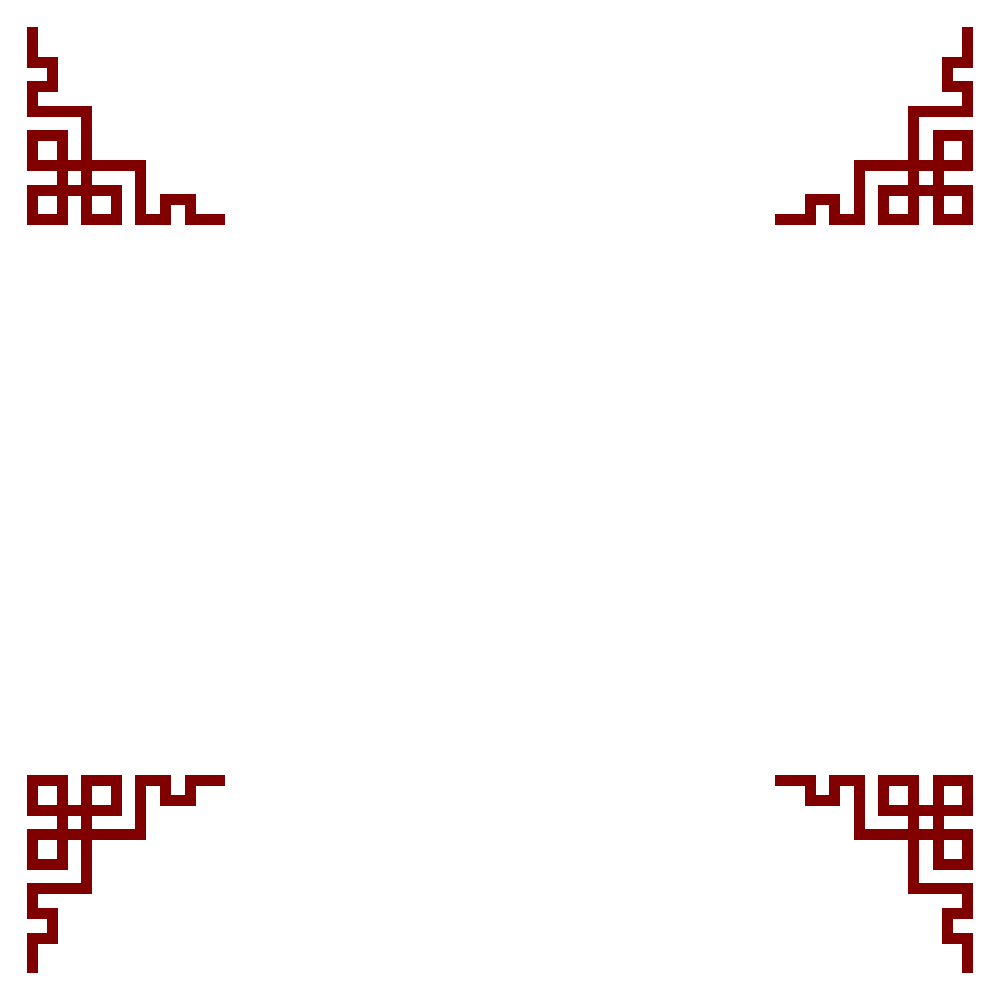
\begin{tikzpicture}[color=Maroon,
        every node/.style={inner sep=0pt}]
        \node[minimum size=12cm](vecbox){%
            \begin{minipage}{\textwidth}
            \centering
        \BODY
    \end{minipage}};
        \node[anchor=north west] at (vecbox.north west)
        {\pgfornament[width=2.5cm,symmetry=h]{3}};
        \node[anchor=north east] at (vecbox.north east)
        {\pgfornament[width=2.5cm,symmetry=c]{3}};
        \node[anchor=south west] at (vecbox.south west)
        {\pgfornament[width=2.5cm,symmetry=none]{3}};
        \node[anchor=south east] at (vecbox.south east)
        {\pgfornament[width=2.5cm,symmetry=v]{3}};
        \end{tikzpicture}    
}

\newcommand{\seq}{\texttt{;}}
\newcommand{\paral}{\textbardbl}
\newcommand{\sat}{$\top$}
\newcommand{\unsat}{$\bot$}
\newcommand{\fast}{\texttt{24}}
\newcommand{\inc}{inc}
\newcommand{\uc}{uc\textsuperscript}
\newcommand{\mv}{mv\textsuperscript}
\newcommand{\cloud}{cloud}
\newcommand{\all}{{\footnotesize (\seq,\paral,\sat,\unsat,\fast,\inc,\uc\seq,\uc\paral,\mv)}}
\newcommand{\withtrack}[2]{\textsc{#1}{{\footnotesize (#2)}}}

\newcommand{\MakeOnePage}[4]{
    {\centering
    {
    
    \begin{minipage}{\textwidth}
    \centering
    
    
\begin{tikzpicture}
      \node [circular drop shadow={shadow scale=1.05},
             decorate, decoration=zigzag,
             fill=blue!20,draw,thick,circle,text width=3.5cm,align=center,xshift=2cm]
              {\large\textbf{SMT-COMP\\ 2023}};
    \end{tikzpicture}
    \end{minipage}
    
    \begin{myframe}
    
    \textcolor{red!10!black!90}
    {\Huge #1}\\
    
    \textcolor{green!10!black!90}{
    \large In honor of the results achieved in the SMT-competition}
    
    \medskip
    \ifstrempty{#2}{}{
    \textcolor{red!30!black!90}
    {\textit{Certificate for overall performance}}
    
    
    \textcolor{black}{\large #2}
    
     \medskip
    }

    \ifstrempty{#3}{}{
    \textcolor{red!30!black!90} {\textit{Certificate for divisions}}
    
     \textcolor{black}{\large#3}
    
     \medskip
    }

    \ifstrempty{#4}{}{
     \textcolor{red!30!black!90}  {\textit{Certificate for logic}}
    
     \textcolor{black}{\large #4}
    }
    \vspace{2mm}
    
    
    \vspace{1cm}
    
    {\color{blue!40!black}
    \scalebox{.7}{
    \begin{tabular}{ccccc}
    \cline{1-1} 
    \cline{3-3}
    \cline{5-5}
    \\ \
    Jochen Hoenicke  & &  Bobot François & & Martin Bromberger \\
    Organizer & & Chair & & Organizer \\ 
    \end{tabular}
    }}
    \end{myframe}
    
    }}

}

\begin{document}
\TileWallPaper{4cm}{2cm}{tiling.png}

\MakeOnePage{COLIBRI}{}{}{\withtrack{QF\_FP}{\unsat,\fast}, \withtrack{QF\_FPLRA}{\unsat,\fast}, \withtrack{QF\_ABVFPLRA}{\seq,\paral,\unsat,\fast}}
\newpage
\MakeOnePage{Z3++}{\withtrack{Biggest Lead}{\mv}, \withtrack{Largest Contribution}{\mv}}{\withtrack{QF\_LinearIntArith}{\seq,\paral,\sat,\mv}, \withtrack{QF\_NonLinearIntArith}{\seq,\paral,\sat,\unsat,\fast}, \withtrack{QF\_NonLinearRealArith}{\seq,\paral,\sat}}{\withtrack{QF\_IDL}{\unsat}}
\newpage
\MakeOnePage{OSTRICH}{}{}{\withtrack{QF\_S}{\seq,\paral,\unsat}}
\newpage
\MakeOnePage{SMTInterpol}{\withtrack{Biggest Lead}{\fast}}{\withtrack{QF\_Datatypes}{\fast,\uc\textsuperscript\paral}, \withtrack{QF\_Equality+LinearArith}{\seq,\paral,\sat,\inc,\mv}, \withtrack{QF\_NonLinearIntArith}{\inc}}{\withtrack{QF\_UFDT}{\uc\textsuperscript\seq}, \withtrack{QF\_UFDTLIA}{\unsat,\fast,\uc}, \withtrack{QF\_LIA}{\unsat}, \withtrack{QF\_AUFNIA}{\seq,\paral,\sat,\unsat,\fast,\uc}, \withtrack{ALIA}{\sat,\uc}, \withtrack{QF\_ANIA}{\seq,\paral,\sat,\unsat,\fast,\inc,\uc}, \withtrack{QF\_ALIA}{\uc}, \withtrack{UFLIA}{\sat}, \withtrack{QF\_UF}{\uc\textsuperscript\paral}, \withtrack{UFIDL}{\sat}, \withtrack{AUFDTLIA}{\uc}}
\newpage
\MakeOnePage{Bitwuzla}{\withtrack{Biggest Lead}{\inc}}{\withtrack{QF\_Bitvec}{\inc}, \withtrack{QF\_FPArith}{\seq,\paral,\sat,\unsat,\fast,\inc}, \withtrack{FPArith}{\seq,\paral,\sat,\unsat,\fast,\inc,\uc}, \withtrack{QF\_Equality+Bitvec}{\seq,\paral,\sat,\unsat,\fast,\inc,\mv}, \withtrack{Equality+MachineArith}{\inc}, \withtrack{Bitvec}{\sat}}{\withtrack{QF\_ABVFPLRA}{\uc}, \withtrack{ABVFP}{\sat,\fast}, \withtrack{AUFBV}{\seq,\paral,\sat,\unsat,\fast}, \withtrack{QF\_ABVFP}{\uc}, \withtrack{QF\_BVFPLRA}{\uc}, \withtrack{QF\_BVFP}{\uc}, \withtrack{ABVFPLRA}{\fast}, \withtrack{UFBVFP}{\seq,\paral,\unsat}, \withtrack{AUFBVFP}{\seq,\paral,\sat,\unsat,\fast}, \withtrack{UFBV}{\seq,\paral,\sat,\unsat,\fast}}
\newpage
\MakeOnePage{Vampire}{}{\withtrack{Equality}{\fast}}{\withtrack{UFDTNIA}{\seq,\paral,\unsat,\fast,\uc}, \withtrack{AUFLIA}{\unsat,\fast}, \withtrack{ALIA}{\seq,\paral,\unsat,\fast}, \withtrack{UFDTLIA}{\fast,\uc}, \withtrack{AUFNIRA}{\paral,\unsat,\fast}, \withtrack{UF}{\seq,\paral,\sat}, \withtrack{AUFLIRA}{\fast}}
\newpage
\MakeOnePage{Yices2}{}{\withtrack{QF\_LinearIntArith}{\fast,\inc,\uc}, \withtrack{QF\_Equality+Bitvec}{\uc}, \withtrack{QF\_Equality}{\seq,\paral,\sat,\unsat,\fast,\uc,\mv}, \withtrack{QF\_LinearRealArith}{\seq,\paral,\fast,\uc}, \withtrack{QF\_Bitvec}{\uc}, \withtrack{QF\_Equality+LinearArith}{\fast,\uc}, \withtrack{QF\_Equality+NonLinearArith}{\sat}}{\withtrack{QF\_LIRA}{\seq,\paral,\sat,\unsat,\mv}, \withtrack{QF\_UFLIA}{\unsat,\inc}, \withtrack{QF\_AUFBV}{\fast}, \withtrack{QF\_AUFBVLIA}{\inc}, \withtrack{QF\_UFLRA}{\seq,\paral,\sat,\unsat,\inc,\mv}, \withtrack{QF\_UFNRA}{\seq,\paral,\unsat,\fast,\inc,\mv}, \withtrack{QF\_UFBVLIA}{\inc}, \withtrack{QF\_RDL}{\sat,\unsat,\mv}, \withtrack{QF\_ALIA}{\unsat}, \withtrack{QF\_AUFLIA}{\seq,\paral,\sat,\unsat}}
\newpage
\MakeOnePage{YicesQS}{}{\withtrack{Arith}{\sat,\fast}}{\withtrack{LRA}{\seq,\paral,\unsat}, \withtrack{NRA}{\seq,\paral,\unsat}}
\newpage
\MakeOnePage{STP}{}{\withtrack{QF\_Bitvec}{\seq,\paral,\sat,\unsat,\fast,\mv}}{}
\newpage
\MakeOnePage{Q3B}{}{\withtrack{Bitvec}{\fast}}{}
\newpage
\MakeOnePage{cvc5}{\withtrack{Biggest Lead}{\seq,\paral,\sat,\unsat,\uc}, \withtrack{Largest Contribution}{\seq,\paral,\sat,\unsat,\fast,\inc,\uc}}{\withtrack{QF\_LinearIntArith}{\unsat}, \withtrack{QF\_Strings}{\seq,\paral,\sat,\unsat}, \withtrack{QF\_Datatypes}{\seq,\paral,\sat,\unsat,\uc\textsuperscript\seq}, \withtrack{Equality+MachineArith}{\seq,\paral,\sat,\unsat,\fast,\uc}, \withtrack{Equality}{\seq,\paral,\sat,\unsat,\inc,\uc}, \withtrack{Equality+LinearArith}{\seq,\paral,\sat,\unsat,\fast,\inc,\uc}, \withtrack{Arith}{\seq,\paral,\unsat,\inc,\uc}, \withtrack{QF\_Equality+NonLinearArith}{\seq,\paral,\unsat,\fast,\inc,\uc}, \withtrack{Bitvec}{\seq,\paral,\unsat,\inc,\uc}, \withtrack{QF\_Equality+Bitvec+Arith}{\inc}, \withtrack{Equality+NonLinearArith}{\seq,\paral,\sat,\unsat,\fast,\inc,\uc}, \withtrack{QF\_FPArith}{\uc}, \withtrack{QF\_NonLinearRealArith}{\unsat,\fast}, \withtrack{QF\_Equality}{\inc}, \withtrack{QF\_LinearRealArith}{\unsat}}{\withtrack{QF\_FP}{\sat,\mv}, \withtrack{QF\_IDL}{\uc}, \withtrack{QF\_UFNIA}{\sat}, \withtrack{LIA}{\sat,\fast}, \withtrack{UFDT}{\fast}, \withtrack{QF\_UFLRA}{\uc}, \withtrack{NIA}{\sat,\fast}, \withtrack{QF\_UFDTLIRA}{\seq,\paral,\sat,\unsat,\fast,\uc}, \withtrack{QF\_ALIA}{\inc}, \withtrack{QF\_NIRA}{\seq,\paral,\unsat}, \withtrack{QF\_UFBVDT}{\seq,\paral,\sat,\unsat,\fast}, \withtrack{QF\_AUFLIA}{\uc,\mv}, \withtrack{QF\_BVFPLRA}{\inc}, \withtrack{QF\_AX}{\mv}}
\newpage
\MakeOnePage{OpenSMT}{}{\withtrack{QF\_LinearRealArith}{\sat,\inc,\mv}, \withtrack{QF\_Equality+LinearArith}{\unsat}}{\withtrack{QF\_LIA}{\seq,\paral}, \withtrack{QF\_LRA}{\seq,\paral,\unsat,\fast}, \withtrack{QF\_UFIDL}{\seq,\paral,\sat,\mv}}
\newpage
\MakeOnePage{z3-alpha}{}{\withtrack{QF\_Strings}{\fast}}{\withtrack{QF\_S}{\sat}, \withtrack{QF\_SNIA}{\seq,\paral,\sat}}
\newpage
\MakeOnePage{iProver}{}{}{\withtrack{ANIA}{\unsat}}
\newpage


\end{document}